%%%%%%%%%%%%%%%%%%%%%%%%%%%%%%%%%%%%%%%%%
% Arsclassica Article
% LaTeX Template
% Version 1.1 (1/8/17)
%
% This template has been downloaded from:
% http://www.LaTeXTemplates.com
%
% Original author:
% Lorenzo Pantieri (http://www.lorenzopantieri.net) with extensive modifications by:
% Vel (vel@latextemplates.com)
%
% License:
% CC BY-NC-SA 3.0 (http://creativecommons.org/licenses/by-nc-sa/3.0/)
%
%%%%%%%%%%%%%%%%%%%%%%%%%%%%%%%%%%%%%%%%%

%----------------------------------------------------------------------------------------
%	PACKAGES AND OTHER DOCUMENT CONFIGURATIONS
%----------------------------------------------------------------------------------------

\documentclass[
10pt, % Main document font size
a4paper, % Paper type, use 'letterpaper' for US Letter paper
oneside, % One page layout (no page indentation)
%twoside, % Two page layout (page indentation for binding and different headers)
headinclude,footinclude, % Extra spacing for the header and footer
BCOR5mm, % Binding correction
]{scrartcl}

%%%%%%%%%%%%%%%%%%%%%%%%%%%%%%%%%%%%%%%%%
% Arsclassica Article
% Structure Specification File
%
% This file has been downloaded from:
% http://www.LaTeXTemplates.com
%
% Original author:
% Lorenzo Pantieri (http://www.lorenzopantieri.net) with extensive modifications by:
% Vel (vel@latextemplates.com)
%
% License:
% CC BY-NC-SA 3.0 (http://creativecommons.org/licenses/by-nc-sa/3.0/)
%
%%%%%%%%%%%%%%%%%%%%%%%%%%%%%%%%%%%%%%%%%

%----------------------------------------------------------------------------------------
%	REQUIRED PACKAGES
%----------------------------------------------------------------------------------------

\usepackage[
nochapters, % Turn off chapters since this is an article        
beramono, % Use the Bera Mono font for monospaced text (\texttt)
eulermath,% Use the Euler font for mathematics
pdfspacing, % Makes use of pdftex’ letter spacing capabilities via the microtype package
dottedtoc % Dotted lines leading to the page numbers in the table of contents
]{classicthesis} % The layout is based on the Classic Thesis style


\usepackage[T1]{fontenc} % Use 8-bit encoding that has 256 glyphs

\usepackage[utf8]{inputenc} % Required for including letters with accents

\usepackage{graphicx} % Required for including images
\graphicspath{{Figures/}} % Set the default folder for images

\usepackage{enumitem} % Required for manipulating the whitespace between and within lists

\usepackage{lipsu
m} % Used for inserting dummy 'Lorem ipsum' text into the template

\usepackage{subfig} % Required for creating figures with multiple parts (subfigures)

\usepackage{amsmath,amssymb,amsthm} % For including math equations, theorems, symbols, etc

\usepackage{varioref} % More descriptive referencing

%----------------------------------------------------------------------------------------
%	THEOREM STYLES
%---------------------------------------------------------------------------------------

\theoremstyle{definition} % Define theorem styles here based on the definition style (used for definitions and examples)
\newtheorem{definition}{Definition}

\theoremstyle{plain} % Define theorem styles here based on the plain style (used for theorems, lemmas, propositions)
\newtheorem{theorem}{Theorem}

\theoremstyle{remark} % Define theorem styles here based on the remark style (used for remarks and notes)

%----------------------------------------------------------------------------------------
%	HYPERLINKS
%---------------------------------------------------------------------------------------

\hypersetup{
%draft, % Uncomment to remove all links (useful for printing in black and white)
colorlinks=true, breaklinks=true, bookmarks=true,bookmarksnumbered,
urlcolor=webbrown, linkcolor=RoyalBlue, citecolor=webgreen, % Link colors
pdftitle={}, % PDF title
pdfauthor={\textcopyright}, % PDF Author
pdfsubject={}, % PDF Subject
pdfkeywords={}, % PDF Keywords
pdfcreator={pdfLaTeX}, % PDF Creator
pdfproducer={LaTeX with hyperref and ClassicThesis} % PDF producer
} % Include the structure.tex file which specified the document structure and layout
\usepackage{float}
\usepackage{colortbl}
\hyphenation{Fortran hy-phen-ation} % Specify custom hyphenation points in words with dashes where you would like hyphenation to occur, or alternatively, don't put any dashes in a word to stop hyphenation altogether

%----------------------------------------------------------------------------------------
%	TITLE AND AUTHOR(S)
%----------------------------------------------------------------------------------------

\title{\normalfont\spacedallcaps{Testing of classifiers}} % The article title

%\subtitle{Subtitle} % Uncomment to display a subtitle

\author{\spacedlowsmallcaps{Jan Bielecki}} % The article author(s) - author affiliations need to be specified in the AUTHOR AFFILIATIONS block

\date{} % An optional date to appear under the author(s)

%----------------------------------------------------------------------------------------

\begin{document}

%----------------------------------------------------------------------------------------
%	HEADERS
%----------------------------------------------------------------------------------------

\renewcommand{\sectionmark}[1]{\markright{\spacedlowsmallcaps{#1}}} % The header for all pages (oneside) or for even pages (twoside)
%\renewcommand{\subsectionmark}[1]{\markright{\thesubsection~#1}} % Uncomment when using the twoside option - this modifies the header on odd pages
\lehead{\mbox{\llap{\small\thepage\kern1em\color{halfgray} \vline}\color{halfgray}\hspace{0.5em}\rightmark\hfil}} % The header style

\pagestyle{scrheadings} % Enable the headers specified in this block

%----------------------------------------------------------------------------------------
%	TABLE OF CONTENTS & LISTS OF FIGURES AND TABLES
%----------------------------------------------------------------------------------------

\maketitle % Print the title/author/date block

\setcounter{tocdepth}{2} % Set the depth of the table of contents to show sections and subsections only

\tableofcontents % Print the table of contents

%----------------------------------------------------------------------------------------
%	AUTHOR AFFILIATIONS
%----------------------------------------------------------------------------------------



%----------------------------------------------------------------------------------------
%	INTRODUCTION
%----------------------------------------------------------------------------------------

\section{Introduction}

This report concerns checking the quality of the three classifiers:

\begin{enumerate}[noitemsep] % [noitemsep] removes whitespace between the items for a compact look
\item Multilayer perceptron (MLP) - a class of feedforward artificial neural network.
\item K-Nearest Neighbor (KNN) - classification based on the classes of k-nearest neighbors
\item Support vector machine (SVM) - representation of the examples as points in space, mapped so that the examples of the separate categories are divided by a clear gap that is as wide as possible. New examples are then mapped into that same space and predicted to belong to a category based on which side of the gap they fall.
\end{enumerate}

The data used for calculations are the results of medical examinations for 568 patients diagnosed with cancer. Every record (patient) consists of numerical results of 10 different observables (for example, the number of lymphocytes). For each patient we have information about the type of the tumour (it is benign - class 'B' or malignant - class 'M'). 
 

%------------------------------------------------

\section{Results}

\subsection{Multilayer perceptron}

Description of the experiments for MLP:
\begin{enumerate}[noitemsep] % [noitemsep] removes whitespace between the items for a compact look
\item Each result (recognition error as a function of the epoch) is the average of 100 experimental series
\item Calculations were carried out for different sizes of the hidden layer (5, 6, 7, 8 - these sizes bring the best recognition results)
\item Calculations were carried out for different network training functions (Levenberg-Marquardt backpropagation (lm), Scaled conjugate gradient backpropagation (scg) and BFGS quasi-Newton backpropagation (bfg))
\item Data breakdown ratios: train = 450/568, validate = 59/568, test ratio = 59/568.
\end{enumerate}
The results are presented in Figure~\vref{fig:mlpln}, \vref{fig:mlpscg450} and \vref{fig:mlpbfg} .

\begin{figure}[H]
\centering 
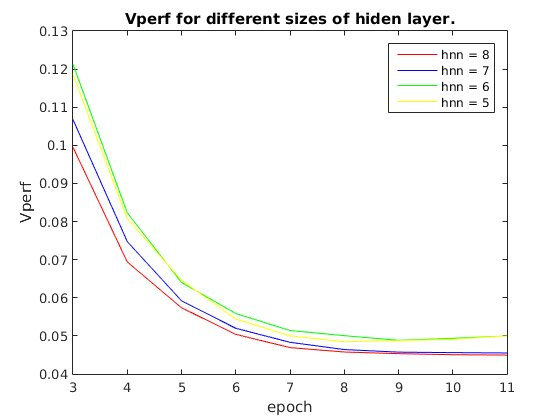
\includegraphics[width=1\columnwidth]{MLP} 
\caption[An example of a floating figure]{Prediction error for MLP method using Levenberg-Marquardt backpropagation (hnn - hidden layer size).} % The text in the square bracket is the caption for the list of figures while the text in the curly brackets is the figure caption
\label{fig:mlpln} 
\end{figure}

\begin{figure}[H]
\centering 
\makebox[\textwidth][c]{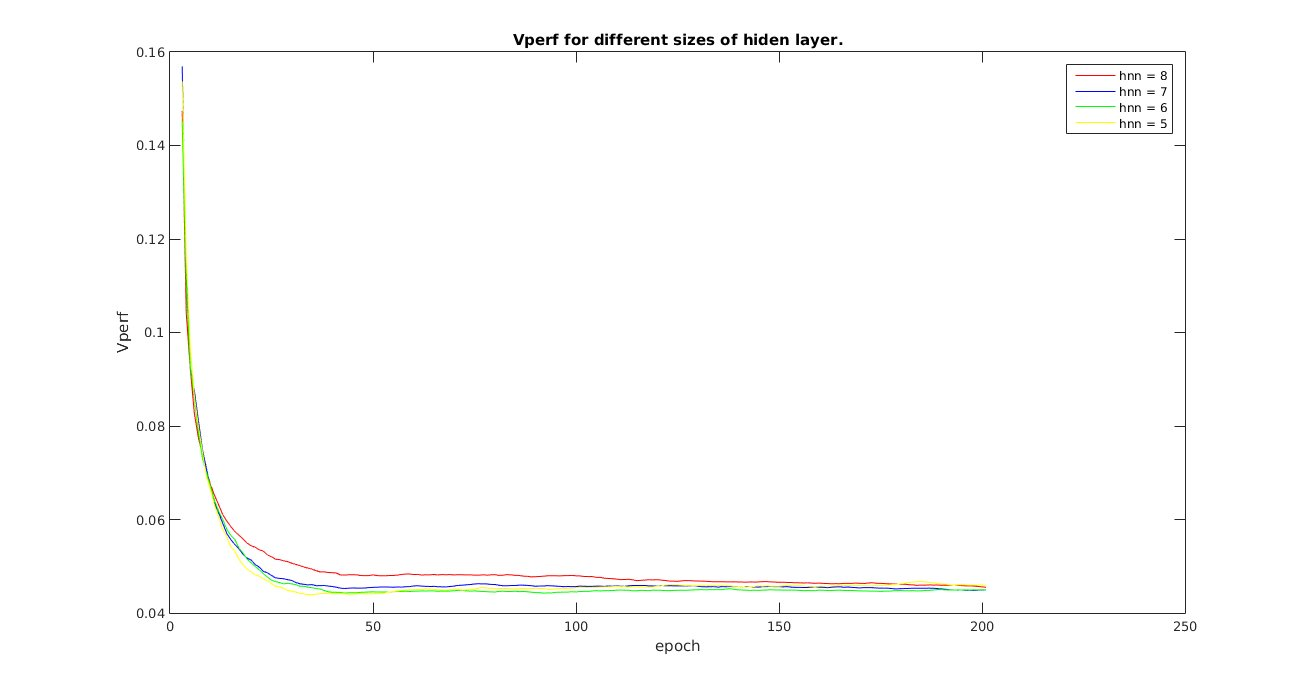
\includegraphics[width=1.5\columnwidth]{MLPscg450}}%
\caption[An example of a floating figure]{Prediction error for MLP method using Scaled conjugate gradient backpropagation (hnn - hidden layer size).} % The text in the square bracket is the caption for the list of figures while the text in the curly brackets is the figure caption
\label{fig:mlpscg450} 
\end{figure}

\begin{figure}[H]
\centering 
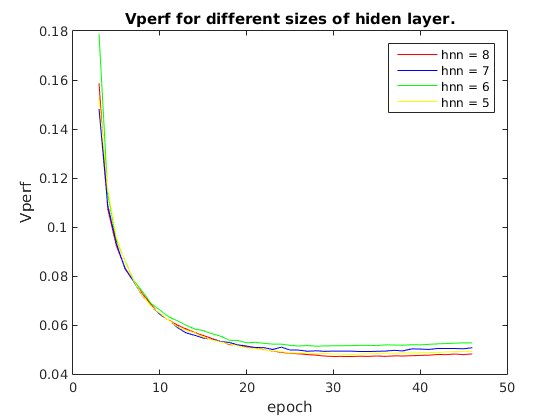
\includegraphics[width=1\columnwidth]{MLPbfg450} 
\caption[An example of a floating figure]{Prediction error for MLP method using BFGS quasi-Newton backpropagation (hnn - hidden layer size).} % The text in the square bracket is the caption for the list of figures while the text in the curly brackets is the figure caption
\label{fig:mlpbfg} 
\end{figure}

\definecolor{amber}{rgb}{1.0, 0.75, 0.0}
\definecolor{antiquebrass}{rgb}{0.8, 0.58, 0.46}
\definecolor{gray(x11gray)}{rgb}{0.75, 0.75, 0.75}

\begin{table}[H]
	\centering
	\begin{tabular}{ | c | c | c | c | c | }
    \hline
     fun/hnn & 5 & 6 & 7 & 8 \\ \hline
    lm & 0.0485 & 0.0488 & 0.0455 & \cellcolor{gray(x11gray)!25}0.0450 \\ \hline
    scg & \cellcolor{amber!25}0.0439 & 0.0443 & 0.0448 & 0.0455 \\ \hline
    bfg & 0.0479 & 0.0513 & 0.0492 & \cellcolor{antiquebrass!25}0.0471 \\ \hline
  	\end{tabular}
  	\caption{Minimum prediction errors for MLP method.}
  	\label{tab1}
\end{table}

Table~\vref{tab1} shows best training results for each training function. % The \vref command specifies the location of the reference

Next, we use 3 and 2 hidden layers with for different sizes and different network's train functions

\begin{table}[H]
	\centering
	\begin{tabular}{ | c | c | c | c | c | c | }
    \hline
    hidden layers & kernel function & series & epochs & $ error_{average,min} $ & $ error_{min} $ \\ \hline
    [8,6,6] & bfg & 100 & 60 & 0.0437 & 0.0031 \\ \hline
    [10,8,6] & bfg & 100 & 60 & 0.0426 & 0.0025 \\ \hline
    [10,8,6] & lm & 100 & 60 & 0.0385 & 0.000093 \\ \hline
    [8,7,6] & lm & 100 & 60 & 0.0419 & \cellcolor{amber!25}0.000091 \\ \hline
    [10,8,6] & scg & 100 & 200 & 0.0420 & 0.0010 \\ \hline
    [8,7,6] & scg & 100 & 200 & 0.0404 & 0.00089 \\ \hline
    [9,7] & lm & 100 & 20 & \cellcolor{amber!25}0.0353 & 0.000071 \\ \hline
  	\end{tabular}
  	\caption{Minimum prediction errors for MLP method.}
  	\label{tab1}
\end{table}

\subsection{K-Nearest Neighbor}

Description of the experiments for KNN:
\begin{enumerate}[noitemsep] % [noitemsep] removes whitespace between the items for a compact look
\item Data (for training the KNN Classifier) have been build with first 450 records
\item Assign the class for each of another 118 records based on k-nearest neibours and find out how much of them has been correctly identified
\item Calculations were carried out for different k parameter (number of nearest neighbors)
\end{enumerate}
The results are presented in Figure~\vref{fig:knn}.

\begin{figure}[H]
\centering 
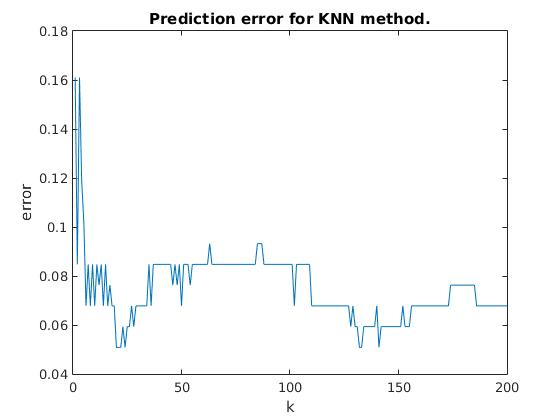
\includegraphics[width=1\columnwidth]{knn} 
\caption[An example of a floating figure]{Prediction error for KNN method (k - number of nearest neighbors).} % The text in the square bracket is the caption for the list of figures while the text in the curly brackets is the figure caption
\label{fig:knn} 
\end{figure}

The best prediction result of KNN method:
\begin{equation}
 error_{MIN} = 0.0471
\label{eq:refname2}
\end{equation}

\subsection{Support vector machine}

Description of the experiments for SVM:
\begin{enumerate}[noitemsep] % [noitemsep] removes whitespace between the items for a compact look
\item Data (for training the SVM Classifier) have been build with first 450 records
\item Assign the class for each of another 118 records based on SVM classifier and find out how much of them has been correctly identified
\item Calculations were carried out for different kernel functions (linear, gaussian, rbf, polynomial)
\end{enumerate}
The results are presented in Table~\vref{tab2}.

\begin{table}[H]
	\centering
	\begin{tabular}{ c | c | c | c | c }
    function  & linear & gaussian & rbf & polynomial \\ \hline
    error & 0.3475 & 0.1271 & 0.1271 & \cellcolor{amber!25}0.1017 \\
  	\end{tabular}
  	\caption{Prediction errors for SVM method.}
  	\label{tab2}
\end{table}

Next, we use principal component analysis for reduce data dimension. Our raw data is 10-dimensional space. We compute principal components for our raw data (using 'princomp' matlab function) and we find out that two components account for 99.99$ \% $ of the variance. The same as before we used 450 records for train and another 118 records for tests.

The minimum prediction error we got by using linear kernel function:

\begin{equation}
 error_{MIN} = 0.1102
\label{eq:refname2}
\end{equation}

\begin{figure}[H]
\centering 
\makebox[\textwidth][c]{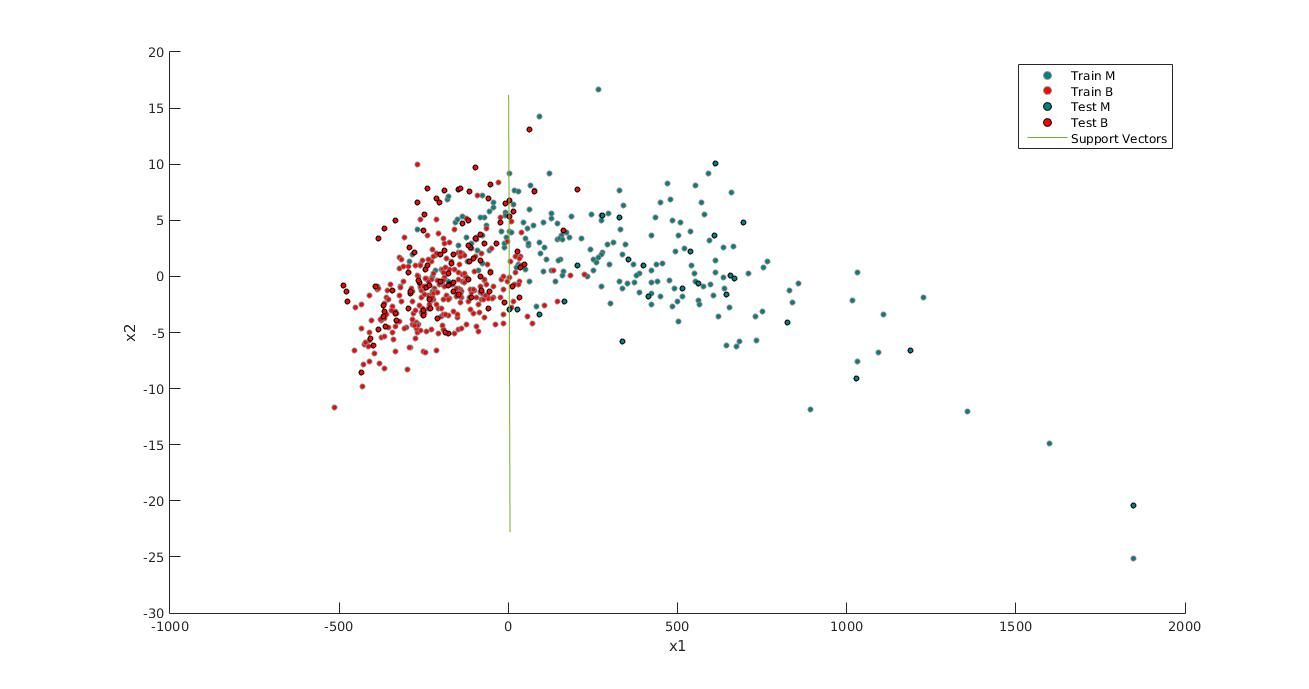
\includegraphics[width=2\columnwidth]{SVM2}}%
\caption[An example of a floating figure]{SVM model for reduced state space.} % The text in the square bracket is the caption for the list of figures while the text in the curly brackets is the figure caption
\label{fig:svm2} 
\end{figure}

Figure~\vref{fig:svm2} illustrates the SVM method for reduced state space (space created using principal component analysis) to two dimensions.

Then we examined SVM method using PCA algoritm for normalize data (Formule~\vref{eq:norm}). Figure~\vref{fig:svmnorm2} illustrates the SVM method using normalized data for reduced state space to two dimensions.

\begin{equation} 
 data(i,j) = \frac{rawData(i,j) - min(rawData(:,j)}{max(rawData(:,j)) - min(rawData(:,j)};
\label{eq:norm}
\end{equation}

\begin{table}[H]
	\centering
	\begin{tabular}{ c | c | c | c | c | c | c | c | c | c | c}
    PCA components  & 1 & 2 & 3 & 4 & 5 & 6 & 7 & 8 & 9 & 10 \\ \hline
    $ \% $ of the variance & 61 & 83 & 90 & 95 & 97 & 99 & 99 & 100 & 100 & 100 \\
  	\end{tabular}
  	\caption{Percent of the data variance depending on the number of principal components.}
  	\label{tab2}
\end{table}

\begin{table}[H]
	\centering
	\begin{tabular}{ c | c | c | c | c }
    PCA components/Kernel function & linear & gaussian & rbf & polynomial \\ \hline
    2 & 0.0932 & 0.2373 & 0.2373 & 0.2542 \\ \hline
    3 & \cellcolor{amber!25}0.0424 & 0.1186 & 0.1186 & 0.3559 \\ \hline
    4 & \cellcolor{amber!25}0.0424 & 0.1102 & 0.1102 & 0.2542 \\ \hline
    5 & 0.2881 & 0.1186 & 0.1186 & 0.1695 \\ \hline
    6 & 0.1186 & 0.1441 & 0.1441 & 0.1780 \\ \hline
    7 & 0.1864 & 0.1186 & 0.1186 & 0.1780 \\
  	\end{tabular}
  	\caption{Prediction error for SVM method for different parameters.}
  	\label{tab2}
\end{table}

\begin{figure}[H]
\centering 
\makebox[\textwidth][c]{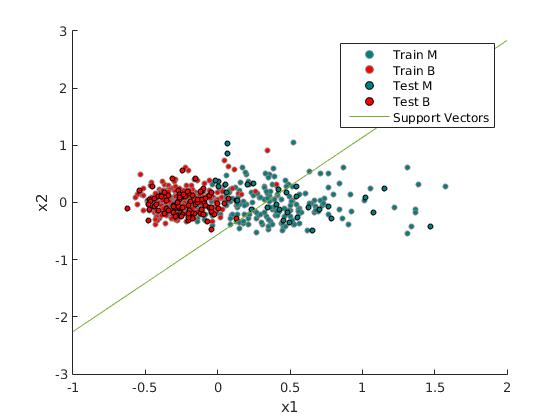
\includegraphics[width=1.3\columnwidth]{SVMNorm2}}%
\caption[An example of a floating figure]{SVM model for normalized data and reduced state space.} % The text in the square bracket is the caption for the list of figures while the text in the curly brackets is the figure caption
\label{fig:svmnorm2} 
\end{figure}


%----------------------------------------------------------------------------------------
%	DISCUSSION
%----------------------------------------------------------------------------------------

\section{Discussion}

Table~\vref{tab3} summarizing the best results of the tested classifiers:

\begin{table}[H]
	\centering
	\begin{tabular}{ c | c | c | c  }
    classifier  & MLP & KNN & SVM \\ \hline
    $ error_{MIN} $ & \cellcolor{amber!25}0.0353 & 0.0471 & 0.0424 \\
  	\end{tabular}
  	\caption{Minimum prediction errors of the tested classifiers.}
  	\label{tab3}
\end{table}

For our data the best classification method is  MLP using Levenberg-Marquardt backpropagation as training function. The second best SVM with normalized data using PCA (model with use of 3 or 4 principal components and linear kernel function). The worst of the tested classificators (for our specified data) is KNN method - this classificator got the same results as MLP using BFGS quasi-Newton backpropagation. Moreover, results from the MLP method are averaged and minimum error managed to get from the best configuration is 0.000091.

%----------------------------------------------------------------------------------------
%	BIBLIOGRAPHY
%----------------------------------------------------------------------------------------

\renewcommand{\refname}{\spacedlowsmallcaps{References}} % For modifying the bibliography heading

\bibliographystyle{unsrt}

\bibliography{sample.bib} % The file containing the bibliography

%----------------------------------------------------------------------------------------

\end{document}